% !TEX encoding = UTF-8 Unicode
\setchapterstyle{kao}
\setchapterpreamble[u]{\margintoc}
\chapter{VALIDER UN MODELE}
\labch{valider_un_modele}

\blockquote{En sciences il n'y a pas de résultats irréfutables, il  n'y a que des résultats réfutés.}

La modélisation présente deux fonctions principales : expliquer et prévoir. Cependant toute modélisation repose sur des hypothèses qu'il s'agit de valider. Nous proposons une illustration de l'opération de modélisation et de sa validation scientifique à partir de l'expérience réalisée dans le chapitre précédent sur les oscillations d'un pendule simple. 

\begin{center}
\textbf{Version en ligne}

	\url{https://femto-physique.fr/omp/valider-un-modele.php}
\end{center}


\section{Modélisation}
 
\subsection{Modéliser c'est simplifier}
Tout d'abord, insistons sur les points suivants.
\begin{enumerate}
	\item Toute modélisation repose sur des approximations \emph{dès le départ}.
	\item Ces approximations peuvent concerner le cadre de l'étude. Le fait d'utiliser le cadre de la mécanique newtonienne pour traiter un problème et non la relativité restreinte en est un exemple.
	\item Elles peuvent concerner les phénomènes mis en jeu. Négliger la rotation de la Terre dans l'étude de la chute libre en est une illustration.
\end{enumerate}

Bien entendu les approximations ne sont pas faites au hasard. En général, des considérations expérimentales et/ou théoriques permettent de justifier ces approximations. 

Une fois les hypothèses posées, le physicien cherche à déterminer un modèle (mathématique/numérique) afin de faire des prévisions sur le phénomène. Différentes méthodes s'offrent à lui suivant le point de vue adopté mais dans tous les cas, il est important de comprendre que toute modélisation produit une erreur : c'est le biais théorique.

\subsection{Exemple du mouvement d'un pendule simple}[Exemple du pendule]
Poursuivons notre étude du mouvement d'un pendule simple en proposant un modèle théorique qui permet d'accéder à l'expression de la période $T$ des oscillations en fonction des caractéristiques du pendule. Par la suite, ce modèle sera soumis à l'épreuve des faits.

\textbf{Cadre théorique} -- Plaçons nous dans le cadre de la mécanique classique puisqu'il s'agit de décrire le mouvement d'un corps macroscopique animé d'une vitesse faible devant celle de la lumière.

\textbf{Les hypothèses} -- Simplifions ! Considérons un pendule simple formé d'une bille quasi-ponctuelle de masse $m$, attachée à un fil inextensible de masse négligeable et de longueur $\ell$. Le fil, quant à lui, est fixé en un point O. Écartons le pendule de sa position d'équilibre puis lâchons le. La masse descend et acquiert une énergie cinétique qui la fait remonter. Il est assez clair que l'action du fil et la pesanteur jouent un rôle prépondérant. Cependant, le pendule est soumis à d'autres types d'action. On pourrait citer les frottements de l'air, les effets de la rotation terrestre, les effets électromagnétiques dus au champ magnétique terrestre etc. Négligeons donc ces phénomènes en première hypothèse et nous verrons bien si la précision des mesures permet de réfuter ce modèle. On considère donc un pendule simple soumis uniquement au champ de pesanteur dans un référentiel terrestre galiléen.
\begin{marginfigure}[*0]
\centering
	\begin{tikzpicture} [scale=0.8] 
		\coordinate (O) at (0, 0);
		\coordinate (M) at (-55:5);
		\draw[thick,double=lightgray] (O)node{$\bullet$}node[above right]{O}--(M); 
		\draw (-57:2.5) node[above right]{$\ell$};
		\draw [thin,gray] (-0.5,0)--(5,0); 
		\draw [thin,gray]  (0,0.5) --(0,-6);   
		\draw[vecteur] (O)-- ++(1,0);
		\draw[vecteur] (O)-- ++(0,1);
		\draw (1,0) node[below]  {$\overrightarrow{{u}_{x}}$} ++(-1,1) node[below left]  {$\overrightarrow{{u}_{y}}$};
		\draw[vecteur] (4.5,-1)--++(0,-1) node[midway,right]{$\overrightarrow{g}$};
		\draw[dotted](M)--(0,{-5*sin(55)})node[left]{$y(t)$};
		\draw[dashed](M)++(0,{2*sin(55)})--++({-2*cos(55)},0);
		\draw[dotted](M)--({5*cos(55)},0)node[above]{$x(t)$};
		\draw[dashed](M)++({-2*cos(55)},0)--++(0,{2*sin(55)},0);
		\draw[force] (M)--++({-2*cos(55)},{2*sin(55)}) node[below left]{$\overrightarrow{F}$};
		\draw[->](M)--++(0,{2*sin(55)})node[right]{$\overrightarrow{F}_y$};
		\draw[->](M)--++({-2*cos(55)},0)node[below]{$\overrightarrow{F}_x$};
		\draw[force] (M)--++(0,-2) node[above right=2pt]{$m\overrightarrow{g}$};
		\draw[bloc] (M) circle(0.2) node[black,right=5pt]{M};
		\draw[->] (0,-1) arc (-90:-55:1);
		\draw (-70:1)node[below=2pt]{$\theta$};
	\end{tikzpicture}
\caption{Bilan des forces}
\labfig{bilan_des_forces}
\end{marginfigure}
\textbf{Détermination de l'équation du mouvement} -- Établissons l'équation du mouvement en projetant les forces et en utilisant la seconde loi de Newton $\overrightarrow{F}=m \overrightarrow{a}$. La masse est soumise à la pesanteur $\overrightarrow{P}=m \overrightarrow{g}$ ainsi qu'à la tension $\overrightarrow{F}$ du fil. Exprimons ces vecteurs dans la base cartésienne :
\[
\overrightarrow{P}=\begin{pmatrix}0\\-mg\end{pmatrix}
\qquad\text{et}\qquad
\overrightarrow{F}=\begin{pmatrix}F_x\\F_y\end{pmatrix}
\]
D'après les relations de Thales on a 
\[\dfrac{F_x}{F}=-\dfrac{x}{\ell}\qquad\text{et}\qquad\dfrac{F_y}{F}=-\dfrac{y}{\ell}	\]
où $F$ désigne l'intensité de la tension du fil. Projetons la seconde loi de newton suivant les axes O$x$ et O$y$ :
\[\left\{\begin{array}{rcccl}
m\ddot y	&=& -mg+F_y	&=& -mg-\dfrac{F}{\ell}y\\[3mm]
m\ddot x	&=& 0+F_x		&=& -\dfrac{F}{\ell}x
\end{array}\right.\]
Par ailleurs, supposons l'angle d'oscillation suffisamment petit de sorte que  $\cos\theta\simeq 1$. En pratique, cela  correspond à des angles inférieurs à 10\(^\circ\) si la précision recherchée est de l'ordre de 1\%. Cela implique 
\[y=-\ell\cos\theta\simeq -\ell  \qquad\text{d'où}\qquad \ddot y \simeq 0 \]
Les équations du mouvement aboutissent à 
\[\left\{\begin{array}{rcl}
F					&=&	mg\\[3mm]
m \ddot x	&=& -\dfrac{mg}{\ell}x
\end{array}	\right.\]
Finalement, le mouvement horizontal est décrit par l'équation 
\begin{equation}
	\ddot x+\frac{g}{\ell}\,x=0
	\label{eq:mouvement_du_pendule_simple}
\end{equation}
Cette équation à pour inconnue \textbf{une fonction} : elle relie une fonction à ses dérivées. Ici l'ordre maximum des dérivées vaut 2 ; on dit qu'il s'agit d'une \textbf{équation différentielle d'ordre 2}. Par ailleurs, on a des contraintes imposées par les conditions initiales 
\[	x(t=0)=x_0 \qquad\text{et}\qquad \dot x(t=0)=0\]
Le nombre de conditions initiales doit toujours être égal à l'ordre de l'équation différentielle (ici 2). Il existe des méthodes analytiques et/ou numériques pour résoudre ce type d'équation différentielle. Ici, on va se servir de notre intuition pour trouver le résultat sachant que la solution est unique. Autrement dit, si l'on trouve une solution alors c'est \emph{la solution}. Compte tenu des oscillations observées, il est légitime de  proposer une solution de la forme $x(t)=a\cos(bt)$ avec $a$ et $b$ des paramètres à déterminer. En premier lieu, la condition initiale $x(0)=x_0$ impose $a=x_0$. Il nous reste à déterminer $b$. Pour cela, remplaçons la  fonction proposée dans l'équation \eqref{eq:mouvement_du_pendule_simple} : si la forme proposée est la bonne, on devrait trouver l'unique valeur de $b$ qui convient.
\[\dfrac{\mathrm{d}^2}{\mathrm{d}t^2}(x_0\cos bt)+\dfrac{g}{\ell}x_0\cos bt=0
\quad\text{d'où}\quad
x_0\cos(bt)\left[-b^2+\dfrac{g}{\ell}\right]=0\]
équation qui n'est vérifiée que si $b=\sqrt{g/\ell}$. L'unique solution de notre équation est donc \[x(t)=x_0\cos\sqrt{\frac{g}{\ell}}t\]
Il nous reste à déterminer la période $T$ des oscillations. Le pendule passe à la verticale quand $x(t)=0$ soit
\[\cos\sqrt{\frac{g}{\ell}}\,t=0 
\quad\Longrightarrow\quad \sqrt{\frac{g}{\ell}}\,t_k=\pi/2+k\pi 	\]
Par conséquent, la période des oscillations vaut 
\begin{equation}
	T=2(t_1-t_0)=2\pi\sqrt{\frac{\ell}{g}}
\label{eq:periode_pendule_simple}
\end{equation} 

\textbf{Analyse du résultat} -- Notons que l'on trouve une relation qui a la forme prévue par l'analyse dimensionnelle effectuée au \refch{unites_et_dimensions}. Elle est donc nécessairement homogène.

Il est bon, lorsque l'on obtient un résultat théorique, d'en analyser le contenu. Ici, la formule \eqref{eq:periode_pendule_simple} nous «dit» que la période augmente avec $\ell$. C'est effectivement ce que l'on observe. Par ailleurs, elle affirme que plus le champ de pesanteur est grand plus la période diminue ce qui semble logique puisque plus le champ de pesanteur est grand et plus la bille tombe vite. En revanche, la masse n'intervient pas dans la formule comme nous l'avions prévu dans l'analyse dimensionnelle. Rien d'étonnant si l'on se souvient que la chute libre est indépendante de la masse.

Enfin, n'oublions pas que le modèle est une simplification, ce qui signifie que le résultat a un domaine de validité restreint :
\begin{enumerate}
	\item la masse ne doit pas être trop grande sinon le fil s'allonge périodiquement et $\ell$ n'est alors plus constant ;
	\item la masse ne doit pas être trop petite sinon celle du fil n'est plus négligeable ;
	\item la longueur ne doit pas être trop petite sinon la vitesse est grande d'où des frottements qui peuvent devenir non négligeables ;
	\item l'angle initial doit rester petit.
\end{enumerate}


\section{Comparer deux valeurs}
\begin{margintable}[*3]
\centering
\footnotesize
\begin{tabular}{l|cc}
$\ell$ [cm]	& 70,0~$\pm$~0,1			& 48,0~$\pm$~0,1 \\
\midrule
$T$ [s]		&1,67~$\pm$~0,03	& 1,38~$\pm$~0,06
\end{tabular}
\caption{Mesure de la période du pendule simple pour deux longueurs différentes.}
\labtab{mesure_de_periode_pour_deux_longueurs}
\end{margintable}
Toute prédiction théorique doit être mise à l'épreuve des faits avant d'être validé. Illustrons cette  étape sur les oscillations du pendule simple dont une modélisation aboutit au résultat théorique
\[T=2\pi\sqrt{\frac{\ell}{g}}\]
et confrontons celui-ci aux mesures que donne une série d'expériences (cf. \reftab{mesure_de_periode_pour_deux_longueurs}). Ici, les deux mesures indépendantes doivent fournir deux valeurs compatibles de $g$.

\subsection{Généralités} % (fold)
Comparer deux valeurs expérimentales c'est se poser la question suivante : l'écart entre ces deux valeurs est-il \textbf{significatif} ? En d'autres termes, on se demande si l'écart est lié aux erreurs aléatoires de mesure auquel cas l'écart est non significatif. Sinon l'écart est significatif et traduit une \textbf{différence objective}.
\begin{figure}[h!tbp]
	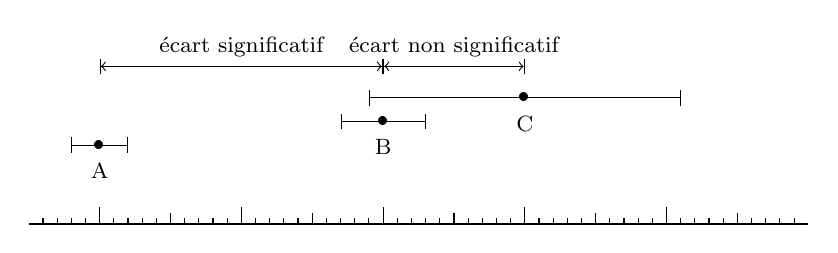
\begin{tikzpicture} [xscale=1.8,font=\footnotesize] 
	\draw[thick] (-0.5,-1)--++(5.5,0);
	\foreach \x in {-0.4,-0.3,...,4.9}
	     		\draw[shift={(0,-1)},thin] (\x,0) --++ (0,2pt);
	\foreach \x in {0,0.5,...,4.5}
	     		\draw[shift={(0,-1)},thin] (\x,0) -- (\x,4pt);
	\foreach \x in {0,...,4}
	     		\draw[shift={(0,-1)}] (\x,0) -- (\x,6pt);
	\draw[|-|] node{•}node[below=3pt]{A}++(0.2,0)--++(-0.4,0);
	\draw[|-|,shift={(2,0.3)}] node{•}node[below=3pt]{B}++(0.3,0)--++(-0.6,0);
	\draw[|-|,shift={(3,0.6)}] node{•}node[below=3pt]{C}++(1.1,0)--++(-2.2,0);
	\draw[|<->|,shift={(0,1)}] (0,0)--++(2,0) node[above,midway]{écart significatif};
	\draw[|<->|,shift={(0,1)}] (2,0)--++(1,0) node[above,midway]{écart non significatif};
	\end{tikzpicture}
	\caption{A et B sont \emph{significativement} différents contrairement à B et C.}
\end{figure}
La difficulté réside dans le fait que nous ne connaissons pas les valeurs vraies des quantités que l'on mesure mais simplement des intervalles de confiance. En pratique, considérant qu'un niveau de confiance de 95\% est suffisant, on regarde si les deux intervalles de confiance se chevauchent : si oui, il n'y a pas de désaccord significatif.

Par ailleurs, on peut être amené à comparer une valeur expérimentale avec une valeur tabulée (intensité de la pesanteur, chaleur latente de fusion de l'eau, charge de l'électron, etc.). En général, ces valeurs ne sont pas exactes\sidenote{Il existe toutefois quelques grandeurs dont on connaît les valeurs exactes de par les définitions des unités. Par exemple la célérité de la lumière dans le vide $c$, le nombre d'Avogadro et la constante de Planck ont des valeurs exactes dans le nouveau Système international d'unités.} puisqu'elles sont entachées d'une incertitude. Néanmoins, ces valeurs sont beaucoup plus précises que celles obtenues dans le cadre des Travaux Pratiques, c'est pourquoi on considère les valeurs tabulées comme des valeurs exactes.
\begin{kaobox}[frametitle=À retenir]
\begin{itemize}
	\item Deux résultats sont significativement différents si leur marge d'erreur à 95\% de niveau de confiance ne se recouvrent pas.
	\item Un résultat expérimental est différent d'une valeur tabulée si cette dernière est située en dehors de la marge d'erreur à 95\%.
\end{itemize}
\end{kaobox}

% (end)


\subsubsection{Que faire s'il y a un désaccord significatif ?}
Un désaccord significatif impose d'en chercher l'origine. Cet exercice peut s'avérer délicat, comme nous le rappelle la célèbre affaire des neutrinos supraluminiques. En général, il faut explorer trois pistes.
\begin{description}
	\item[L'erreur de calcul --] On n'est jamais à l'abris d'erreur de saisie sur la calculatrice ou le tableur. De plus, on peut aussi avoir mal calculé les incertitudes. 
	\item[La présence de biais expérimentaux --] Il se peut qu'une erreur systématique non détectée soit responsable de ce désaccord. Par exemple, un chronomètre décalibré, un étalonnage mal fait etc.
	\item[Remettre en cause le modèle --] Comme on l'a vu, tout modèle repose sur des hypothèses simplificatrices. Il se peut que les effets de ces simplifications ne soient pas négligeables compte tenu de la précision des mesures. Il faut alors raffiner le modèle pour décrire plus fidèlement la réalité.
\end{description}


\subsection{Exemple}
Reprenons l'expérience des oscillations d'un pendule simple. On a établit un résultat théorique qui montre que la mesure de la période du pendule permet de mesurer le champ de pesanteur. Commençons donc par calculer les valeurs de $g$ à partir des deux mesures. On a la relation 
\[g=4\pi^2\frac{\ell}{T^2}\]
ce qui permet d'exprimer l'incertitude $\Delta g$ à partir des incertitudes sur la longueur et la période du pendule simple.\begin{margintable}
\centering
\caption{Résultats expérimentaux.}
\labtab{resultats_experimentaux}
\footnotesize
\begin{tabular}{l|cc}
\toprule
$\ell$ [cm]	& 70,0~$\pm$~0,1			& 48,0~$\pm$~0,1 \\[1mm]
$T$ [s]		&1,67~$\pm$~0,03	& 1,38~$\pm$~0,06\\[1mm]
$g$ [m.s$^{-2}$]	&9,9~$\pm$~0,4	& 10,0~$\pm$~0,9\\
\bottomrule
\end{tabular}
\end{margintable} On a 
\[\begin{array}{rcl}\dfrac{\partial g}{\partial \ell}	&=&\dfrac{4\pi^2}{T^{2}}\\[3mm]
\dfrac{\partial g}{\partial T}	&=& -\dfrac{8\pi^2\,\ell}{T^{3}}\\
\end{array}
\quad\Longrightarrow\quad
\mathrm{d}g=4\pi^2\,T^{-2} \mathrm{d}\ell-8\pi^2\,\ell\,T^{-3} \mathrm{d}T\]
de sorte que l'incertitude sur $g$ vaut 
\[\Delta g = \sqrt{(4\pi^2\,T^{-2}\Delta\ell)^2+(8\pi^2\,\ell\,T^{-3}\Delta T)^2}\]
Consignons nos résultats dans la \reftab{resultats_experimentaux}.
\begin{marginfigure}
\centering
 	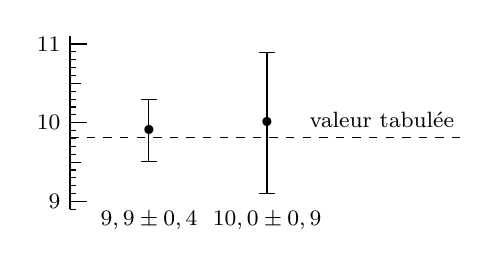
\begin{tikzpicture} [font=\footnotesize] 
 	\draw[thick] (-1,8.9)--++(0,2.2);
 	\foreach \y in {8.9,9,...,11.1}
 	   	\draw[shift={(-1,0)},thin] (0,\y) -- (2pt,\y);
 	\foreach \y in {9.5,10.5}
 	   	\draw[shift={(-1,0)},thin] (0,\y) -- (4pt,\y);
 	\foreach \y in {9,10,11}
 	   	\draw[shift={(-1,0)}] (0,\y) node[left]{\y}-- (6pt,\y);
 	\draw[|-|,shift={(0,9.9)}] node{\(\bullet\)}++(0,0.4)--++(0,-0.8);
 	\draw (0,9)node[below]{$9,9\pm0,4$};
 	\draw[|-|,shift={(1.5,10)}] node{\(\bullet\)}++(0,0.9)--++(0,-1.8);
 	\draw (1.5,9)node[below]{$10,0\pm0,9$};
 	\draw[dashed](-1,9.81)--++(5,0)node[above left]{valeur tabulée};
 	\end{tikzpicture}
  \caption{Représentation graphique des résultats.}
\end{marginfigure}
Quant aux tables, elle donnent le champ de pesanteur à Rennes : $g_\text{tab}=9,81\;\mathrm{m.s^{-2}}$. Nos mesures sont donc non seulement compatibles entre elles, mais également avec la valeur tabulée. 



	
\section{Valider une loi}
Décrivons la démarche habituellement employée pour valider une loi à partir de données expérimentales.

\subsection{Régression par la méthode des moindres carrés}[Méthode des moindres carrés]
Supposons que l'on cherche à vérifier une loi du type $y=f(x)$ prévue par un modèle théorique à partir de $n$ mesures $(y_i,x_i)$. Tester la validité de la loi $y=f(x)$ c'est répondre à deux questions :
\begin{enumerate}
	\item Si l'on suppose la loi valide, quelle est la courbe d'ajustement (courbe de régression) qui s'ajuste au plus près des données expérimentales ?
	\item Une fois l'ajustement effectué, peut-on dire si les écarts entre la courbe de régression et les points sont significatifs ? S'ils sont imputables aux erreurs de mesure, alors rien ne permet de réfuter la loi. En revanche, si le désaccord est significatif, il faut en chercher l'origine (problème de calcul, biais expérimental, hypothèses du modèle à réfuter, etc).
\end{enumerate}
\begin{marginfigure}
\centering
	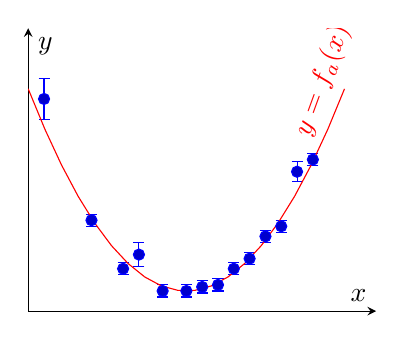
\begin{tikzpicture} 
		\begin{axis}[
		width=6cm,
		axis lines=middle,% bottom,top
		inner axis line style={=>},
		xlabel={$x$},
		ylabel={$y$},
		ymin=0.9,
		ymax=2.3,
		xmin=0,
		xmax=2.2,
		xtick=\empty,
		ytick=\empty,
		]
		\addplot+[only marks,error bars/.cd,y dir=both,y explicit] coordinates {
			(0.1,1.95)+- (0,0.1)
			(0.4,1.35)+- (0,0.03)
			(0.6,1.11)+- (0,0.03)
			(0.85,1) +- (0,0.03)
			(0.7,1.18) +- (0,0.06)
			(1,1)+- (0,0.03)
			(1.1,1.02)+- (0,0.03)
			(1.2,1.03)+- (0,0.03)
			(1.3,1.11)+- (0,0.03)
			(1.4,1.16)+- (0,0.03)
			(1.5,1.27)+- (0,0.03)
			(1.6,1.32)+- (0,0.03)
			(1.7,1.59)+- (0,0.05)
			(1.8,1.65)+- (0,0.03)};
		\addplot+[mark=none,domain=0:2,samples=20]{(x-1)^2+1}node[above,rotate=70]{$y=f_\text{a}(x)$};
		\end{axis} 
	\end{tikzpicture}
	\caption{Ajustement d'une courbe modèle à un nuage de points expérimentaux.}
\end{marginfigure}
On commence donc par collecter un ensemble de $n$ mesures $(x_i,y_i)$ avec $i=1,\ldots, n$ puis l'on porte les valeurs $y_i$ en fonction de $x_i$.  On obtient  alors un nuage de points. Si on a accès aux incertitudes de mesures, on ajoute alors les \textbf{barres d'erreur}.

Il faut ensuite choisir un \textbf{modèle d'ajustement} $y=f_\text{a}(x)$ qui va dépendre d'un petit jeu de paramètres $a_i$ à déterminer de façon à s'ajuster le mieux possible aux données. Insistons sur un point : le choix du modèle est dicté par la loi théorique que l'on cherche à vérifier. 

\begin{kaoexample}[frametitle=Exemple]
On cherche à vérifier la loi du pendule simple $T=2\pi\sqrt{\ell/g}$. On collecte donc des mesures de la période pour différentes valeurs de $\ell$.
\begin{itemize}
	\item Si l'on porte $y=T$ en fonction de $x=\ell$ on s'attend à trouver une loi du type 
	\[	y=a_1\sqrt{x}\qquad\text{modèle racine carré}\] 
	
	\item On peut aussi porter $y=T$ en fonction de $x=\sqrt{\ell}$. On s'attend à trouver une loi du type 
	\[	y=a_1\,x \qquad\text{modèle linéaire}\]
\end{itemize}
\end{kaoexample} 
Lorsque -- comme c'est le cas dans les exemples précédents -- la fonction à ajuster $f_\text{a}(x)$ est de la forme 
\[
	f_\text{a}(x)=a_1f_1(x)+a_2f_2(x)+\ldots
\]  
On dit alors que l'on fait une \textbf{régression linéaire}.

\textbf{Comment trouver les paramètres d'ajustement ?} -- Cette étape est en général effectuée automatiquement par le logiciel de traitement des données (\texttt{Regressi}, \texttt{Igor}, \texttt{Plot.ly},etc.) et repose sur la \textbf{méthode des moindres carrés} (\emph{least squares fitting} en anglais). Cela consiste à rechercher la valeur des paramètres qui minimise la somme des écarts quadratiques entre les mesures $y_i$ et les valeurs attendues $f_\text{a}(x_i)$. Si les incertitudes sont fournies, on pondère les écarts de façon à ce que les points les plus précis aient plus d'importance dans la somme à minimiser. On définit alors 
\[
	\chi^2(a_i)=\sum_i \frac{(y_i-f_\text{a}(x_i))^2}{{\Delta y_i}^2}
\]
Cette somme dépend des paramètres $a_i$. Le logiciel calcule les valeurs des paramètres qui rend $\chi^2$ minimum. Une fois ces paramètres calculés, on peut tracer la courbe modèle et vérifier si elle passe par les barres d'erreur.


\subsection{Utilisation de \texttt{Regressi}}
Illustrons le principe de la régression avec notre expérience sur les oscillations du pendule simple. Cherchons à vérifier la loi $T=2\pi\sqrt{\ell/g}$ à l'aide du logiciel \texttt{Regressi}.

Une fois le logiciel \texttt{Regressi} lancé, commençons par modifier les options. Notamment, précisons que les incertitudes sont calculés avec les variances puis que l'on utilise la méthode du $\chi^2$ pour l'ajustement. Quant aux graphiques, décidons d'afficher les barres d'erreur avec un niveau de confiance de 95\%.
\begin{figure*}[htbp]
    \includegraphics[width=.45\columnwidth]{img/regressi/option_calcul.JPG}
	\quad
	\includegraphics[width=.45\columnwidth]{img/regressi/options.JPG}
	\caption{copies d'écran de la boite de dialogue \texttt{Option}.}
\end{figure*}

\begin{marginfigure}[*1]
\centering
	\includegraphics[width=5cm]{img/regressi/nouveau_clavier.JPG}
\caption{Entrée des données au clavier.}
\end{marginfigure}
Sélectionnons \fbox{\texttt{Fichier}} $\blacktriangleright$ \texttt{Nouveau}  $\blacktriangleright$  \texttt{clavier}. Le logiciel demande les noms et facultativement les unités ainsi que les intervalles de variation des grandeurs à saisir. Rentrons \texttt{T} pour la période et \texttt{L} pour la longueur. 

Une fois les grandeurs définies, un tableau nous est proposé (onglet \texttt{Variables}). Le remplissage du tableau ne pose pas de difficulté particulière. Pour saisir les incertitudes, il suffit de cliquer sur l'icône \fbox{$\sigma$}. Créons la grandeur $x=\sqrt{\ell}$ en cliquant sur l'icône \fbox{\textbf{Y}$_+$}. Cochons \texttt{Grandeur calc.} puis rentrons la formule \texttt{x=sqrt(L)}. 
\begin{figure}[htbp]
\centering
   \includegraphics[width=\textwidth]{img/regressi/onglet_variables.JPG}	
\caption{Onglet \texttt{variables}. Le logiciel effectue le calcul dans le Système international d'unités si les unités sont fournies. Ici, on a indiqué les unités de \texttt{L} en cm de sorte que, lors du calcul de $x$, \texttt{L} est converti en mètre.}
\end{figure}

Ouvrons la fenêtre graphique en sélectionnant l'onglet \texttt{Graphe}. Pour spécifier les variables en abscisse et en ordonnées il suffit de sélectionner \texttt{Coordonnées} après un clic-droit sur le graphe. Une boîte de dialogue permet alors de régler les coordonnées, l'échelle, le lissage, le type de tracé etc. Pour afficher les barres d'erreur, choisir \texttt{Incertitudes} dans l'option d'affichage des points. On porte \texttt{T} en fonction de \texttt{x}.	

On cherche à tester la loi $y=a\,x$. Pour cela, ouvrons l'espace dédié aux ajustements en cliquant sur \fbox{\texttt{modélisation}} $\blacktriangleright$ \texttt{modèles} puis choisissons un modèle linéaire. Terminons en cliquant sur \texttt{Ajuster} : le logiciel recherche le meilleur ajustement en fonction des données. Comme l'indique la figure~\ref{fig:fig_regression}, La droite d'ajustement passe à travers les barres d'erreur. Autrement dit, \textbf{les écarts à la loi sont non significatifs mais liés aux erreurs de mesure} et la loi est validée.
\begin{figure}[ht]
  \centering
    \includegraphics[width=\textwidth]{img/regressi/regression.JPG}
  \caption{Résultat de l'ajustement sous \texttt{Regressi}}
  \label{fig:fig_regression}
\end{figure}

En prime, on accède au coefficient directeur de la droite avec son incertitude (à 95\% de  niveau de confiance):
\[
	a=2,00\pm 0,02\;\mathrm{s.m^{-1/2}}
\]
Or, la théorie prévoit $a=2\pi/\sqrt g$ ce qui permet d'obtenir une nouvelle valeur de $g$ :
		\[g=\frac{4\pi^2}{a^2}=9,87\;\mathrm{m.s^{-2}}
		\quad\text{et}\quad
		\frac{\Delta g}{g}=2\frac{\Delta a}{a}=2\%
		\] 
Ainsi, nos mesures valident notre modèle et aboutissent à une détermination de $g$ :
\[
	g=9,9\pm0,2\;\mathrm{m.s^{-2}}
\]
